\documentclass[diss-proposta,nocipinfo]{texufpel}
%nocipinfo para não aparecer os dados da CIP no Resumo

\usepackage[utf8]{inputenc} % acentuacao
\usepackage{graphicx} % para inserir figuras
\usepackage[T1]{fontenc}

\hypersetup{
    hidelinks, % Remove coloração e caixas
    unicode=true,   %Permite acentuação no bookmark
    linktoc=all %Habilita link no nome e página do sumário
}

\unidade{Centro de Desenvolvimento Tecnológico}
\programa{Programa de Pós-Graduação em Computação}
\curso{Ciência da Computação}

\title{Estudo e Revisão das Técnicas de Mineração de Dados em Ambientes Educacionais}

\author{Costa}{Alexandre Gomes da}
\advisor[Prof.~Dr.]{Mattos}{Julio Carlos Balzano de}
\coadvisor[Prof.~Dr.]{Primo}{Tiago}

%Palavras-chave em PT_BR
\keyword{mineração de dados educacionais}
\keyword{learning analytics}
\keyword{técnicas de predição}
\keyword{kdd}
\keyword{descoberta de conhecimento em base de dados}

%Palavras-chave em EN_US
\keywordeng{educational data mining}
\keywordeng{learning analytics}
\keywordeng{prediction techniques}
\keywordeng{kdd}
\keywordeng{knowledge-discovery in databases}


\begin{document}

\maketitle 
\sloppy

%Resumo em Portugues (no maximo 1 pagina)
\begin{abstract}
Uma grande quantidade de dados vem sendo produzida através de diversas modalidade de iteração em sistemas envolvendo alunos e professores. Contudo, grande parte desses dados não sofre qualquer tipos de analise. Nos últimos anos uma gama cada vez maior de trabalhos vem surgindo na área de Mineração de Dados Educacionais (MDE). Devido a essa grande quantidade de trabalhos é que se faz necessário fazer um levantamento para descobrir quais métodos, técnicas e algoritmos vem sendo utilizado, e ainda quais tipos de problemas vem sendo apurados. A pesquisa foi realizada, procurando responder as seguintes questões: Qual tem sido as técnicas utilizadas nos trabalhos na área. Qual tipo de dados estão sendo considerados pertinentes na área. Qual é o objetivo de estudo dos trabalhos na área. Qual são as ferramentas que tem sido utilizadas na área. O objetivo deste trabalho é fazer uma busca nas principais meios de publicações brasileiros que vem pesquisando MDE utilizando técnicas de predição.
\end{abstract}

\chapter{Motivação}
% (ENTRE 1 e 2 PÁGINAS)

% Nesta seção, apresenta-se um breve histórico da área de concentração
% da Dissertação, partindo do tema mais abrangente até chegar
% especificamente no assunto do Projeto. Além disso, apresenta-se a
% justificativa para a realização do trabalho, sua importância acadêmica
% ou para comunidade e grau de inovação. Poderá também apresentar as
% distinções entre o trabalho atual e outros trabalhos já realizados.

*** Motivação: dados evasão do INEP, motivar o trabalho (já está) e colocar os trabalhos relacionados (para embasar o trabalho)
Sequencia: evasão, etc -> TICs - TICs na evasão -> objetivo (teu trabalho)
1. Crescimento da Educação Superior
2. Taxas evasão, trancamento elevadas
3. Isto é um problema !
4. TICs
5. TICs no ambiente educacional (evasão)


*** Metodologia

http://portal.inep.gov.br/web/guest/sinopses-estatisticas-da-educacao-superior

INSTITUTO  NACIONAL  DE  ESTUDOS  E  PESQUISAS  EDUCACIONAIS  ANÍSIO  TEIXEIRA. 
Sinopse Estatística da Educação Superior 2016. Brasília: Inep, 2017. Disponível  em:  <http://portal.inep.gov.br/web/guest/sinopses-estatisticas-da-educacao-superior>. Acesso em: dd mm. yyyy.  


O uso constante de Tecnologia da Informação e Comunicação em diversas áreas vem gerando um grande volume de dados.
Tecnologias como a internet, redes sociais, ambientes virtuais de aprendizagem, dispositivo móveis, aplicativos embarcados, leitores de código de barras, sensores, leitores biométricos e sistemas de informação em geral são alguns exemplos de recursos que vem aumentando o numero de dados das mais diversas naturezas \cite{goldschmidt2015data}.

%% Educação
Atualmente, áreas como a educação produzem dados relacionados a alunos e professores todos os dias.
Necessidades da educação como sistemas para fazer o controle de iterações acadêmicas, gestão de projetos de pesquisa, ensino ou extensão, ou até mesmo sistemas para fazer o controle de gestão de pessoas são alguns do exemplos de sistemas que podem gerar um volume considerável de dados com frequência.

%% Knowledge Discovery in Database - KDD
Embora com ajuda de ferramentas computacionais, analisar essa crescente quantidade de dados não é trabalho para o homem \cite{goldschmidt2015data}. Para ajudar nesta questão a área de Descoberta de Conhecimento em Base de Dados (\textit{Knowledge Discovery in Database} - KDD) é focada em extrair conhecimento encima de granes volumes de dados. O termo mais conhecido relacionado a essa área é a Mineração de Dados (MD) que é uma das etapas do processo de KDD.

%% Mineração de dados educacionais
Segundo \citet{Koedinger2008} Mineração de Dados (MD) aplicada à educação é um campo interdisciplinar emergente mais conhecido como Mineração de Dados Educacionais (MDE).
\citet{baker2010data} define MDE como a área de investigação científica centrada no desenvolvimento de métodos para fazer descobertas dentro dos tipos de dados que vêm de ambientes educacionais e usando esses métodos para entender melhor os alunos e a aprendizagem deles. A Figura \ref{fig:areas-relacionadas-mde} mostra que a área de MDE pode ser a combinação de 3 grandes áreas (ciência da computação, estatistia e educação) e serve de exemplo para justificar a interdisciplinaridade da área.

\begin{figure}[htbp]
  \centering 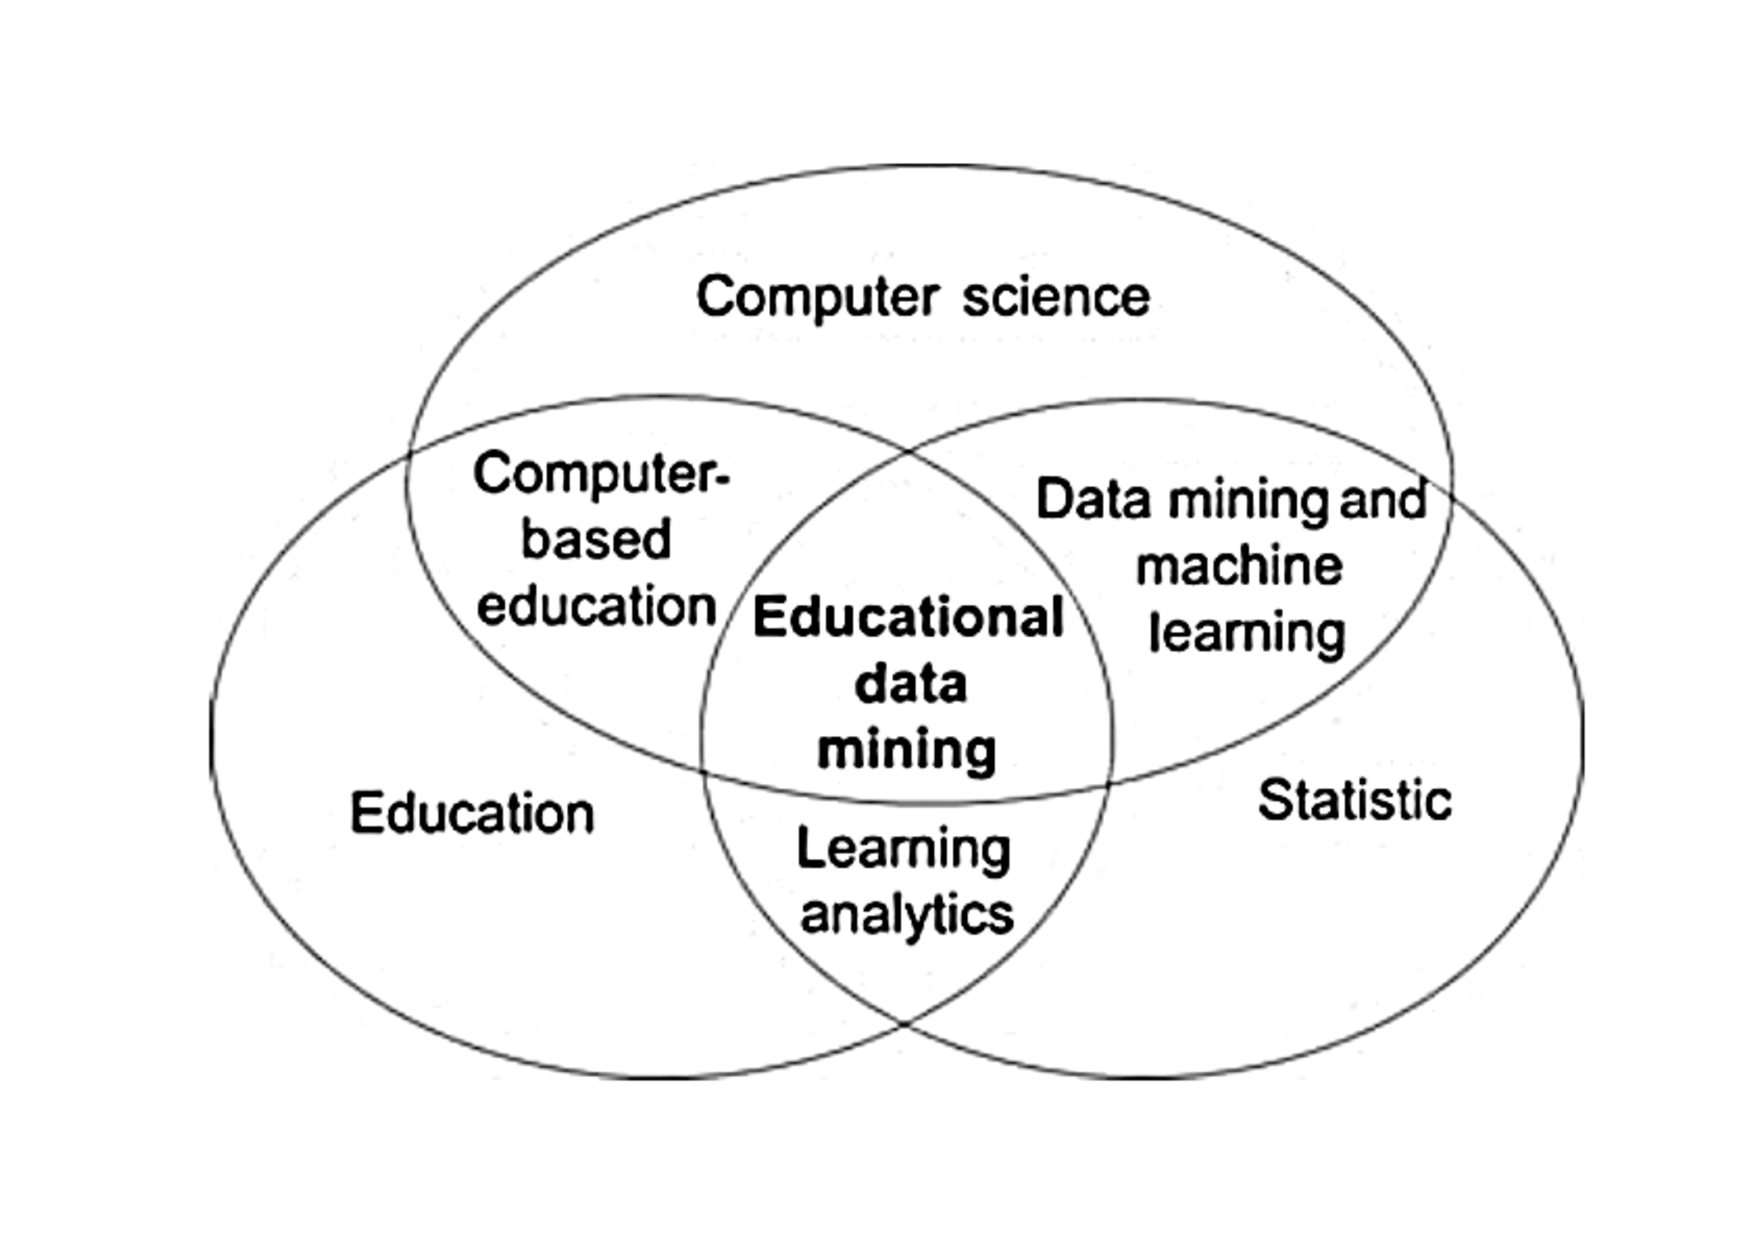
\includegraphics[scale=.4]{imagens/areas-edm.pdf}
  \caption{Principais áreas relacionadas com mineração de dados educacionais. \cite{Koedinger2008}}
  \label{fig:areas-relacionadas-mde}
\end{figure}


%% Predição
Neste trabalho será aplicado um tarefa de classificação para tentar resolver o problema de evasão escolar. 
Segundo \citet{goldschmidt2015data} uma tarefa de classificação possui dois grupos. Um grupo contem normalmente um atributo apenas que vai servir para fazer a predição de um valor (atributo-alvo). Outro grupo corresponde aos atributos que vão servir para fazer a predição do valor (atributos de predição).
Tarefas de classificação são largamente utilizadas para fazer a predição de alunos em risco de evasão escolar, como será apresentado mais afrente.

\citet{baker2010data} agrupa o problema de evasão em uma categoria ou tarefa de detectar o comportamento do aluno.
Onde o objetivo é detectar os alunos que têm algum tipo de problema ou comportamento incomum, por exemplo: ações erradas, pouca motivação, trapaça, evasão escolar, etc.
Destaca também que as principais técnicas usadas para resolver esses tipos de problemas são de classificação e agrupamentos.

%% Justificativa
Este trabalho busca usar a base de dados do Cobalto que é o Sistema Integrado de Gestão da UFPEL. A base do Cobalto conta também com os dados históricos do GOL que foi o sistema acadêmico da UFPEL de 2006 à 2013. %% CONTINUAR

A grande vantagem deste estudo está na naturalidade dos dados. Quanto alguns trabalhos fazem questionários, provas, exercícios, etc, no presente trabalho serão coletado dados que foram gerados a partir de resultado que os alunos obtiveram em diversas disciplinas e cursos.

%% Importância acadêmica


%% Distinções entre o trabalho atual e os trabalhos já realizados

\chapter{Objetivos e Resultados}
% (ENTRE 1 e 3 PÁGINAS)

Este trabalho tem como objetivo estudar e aplicar técnicas de KDD aos dados do sistema Cobalto, para obter um padrão de predição da evasão de alunos através de dados inerentes aos estudantes da UFPEL. Para atingir este objetivo é preciso dividir o trabalho em objetivos específicos.

O primeiro objetivo específico é investigar o que esta sendo pesquisado na área de mineração de dados educacionais, tentando focar em trabalho que tratam da evasão de alunos.

Em seguida é preciso fazer um levantamento do referencial teórico e apresentar os principais conceitos a repeito de mineração de dados educacionais. Mais especificamente seria estudar e apresentar os conceitos de KDD, mineração de dados e mineração de dados educacionais.

Por fim, criar e testar modelos de predição de alunos em risco de evasão de estudantes da UFPEL, utilizando os dados acadêmicos dos alunos.

Em geral a grande maioria dos trabalho com este foco utilizam base de dados de sistemas de EAD. O grande diferencial deste trabalho é que será utilizado um base de dados histórica consolidada de alunos da UFPEL.

Espera-se que os resultados deste trabalho seja aplicado ao sistema acadêmico da UFPEL para ajudar discentes e docentes a prever e combater a evasão.

% Nesta seção, apresentam-se o objetivo Geral e os objetivos Específicos
% da dissertação. Os objetivos não devem ser confundidos com as
% atividades. Para a definição das atividades, deve-se partir dos
% objetivos determinados nesta seção. O objetivo Geral do Projeto
% necessariamente deve ser algum resultado prático (implementação) ou
% teórico (modelos formais ou especificações ou validações) produto da
% pesquisa realizada no período do Projeto. Assim como os objetivos
% específicos, que são considerados como sub-produtos do Objetivo
% Geral. Além disso, deve-se apresentar os principais resultados
% esperados do desenvolvimento desta dissertação.

\chapter{Metodologia}
% (ENTRE 1 e 3 PÁGINAS)

% O processo de mineração de dados envolve várias fases e etapas. Este trabalho classifica o processo de KDD em três grandes fases, com base nas abordagens descritas em [Silva and Vieira 2002] e [Rezende et al. 2003]: Preparação, Extração de Padrões e Pós-Processamento. Cada fase pode envolver uma ou mais etapas conforme mostra a tabela 1. No entanto, o KDD é um processo iterativo e algumas etapas podem ser realizadas novamente após a análise dos padrões encontrados de forma a melhorá-los \cite{Pimentel2006}.

Neste trabalho será utilizado uma metodologia apresentada no livro de \citet{goldschmidt2015data}, que é baseada na metodologia CRISP-DM (Cross-Industry Standard Process for Data Mining) e em alguns princípios de planejamento de atividades. A metodologia mostrada no livro se difere da metodologia CRISP-DM no momento em que ela sugere aplicar a definição dos objetivos e escolha da técnica de mineração antes da faze de preparação dos dados. Além disso, ela adiciona instrumentos para documentar as decisões e os resultados durante o processo de KDD, um exemplo é o formulário mostrado na figura \ref{fig:formulario-para-documentacao-de-acoes}.

\begin{figure}[htbp]
  \centering 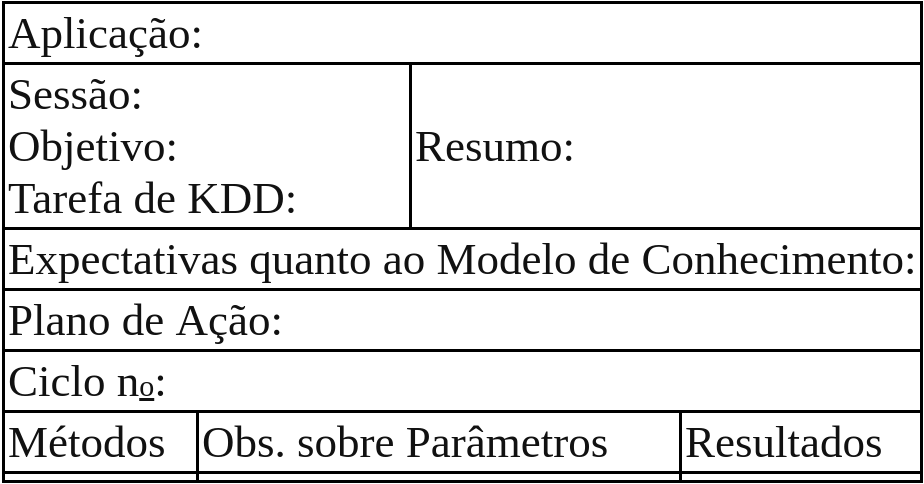
\includegraphics[scale=.4]{imagens/formulario-para-documentacao-de-acoes.png}
  \caption{Formulário para documentação de ações \cite{goldschmidt2015data}.}
  \label{fig:formulario-para-documentacao-de-acoes}
\end{figure}

A metodologia proposta no livo divide o processo em 5 etapas Levantamento da Situação Vigente, Definição dos Objetivos, Planejamento de Atividades, Execução dos Planos de Ação e Avaliação de Resultados. O resto desta sessão aprofunda cada uma dessas etapas.

\section{Levantamento da Situação Vigente}
\label{sec:levantamento-da-situacao-vigente}

Nesta etapa deve ser realizada todas as fases da \textbf{Compreensão do Negócio} e \textbf{Compreensão dos Dados} da metodologia CRISP-DM. 

A fase de \textbf{Compreensão do Negócio} tem como meta compreender o contexto em que o processo de KDD será realizado. As principais considerações técnicas desta fase são:
\begin{itemize}
\item Fazer a identificação das pessoas envolvidas no processo;
\item Elaborar uma lista de necessidades e expectativas das pessoas envolvidas quanto ao propósito do KDD;
\item Conhecer o software e hardware existentes;
\item Elaborar um inventário da base de dados;
\item Verificar se existe um Data Warehouse;
\item Tentar identificar e documentar todo o conhecimento prévio existente e disponível sobre o domínio da aplicação.
\end{itemize}

Na fase de \textbf{Compreensão dos dados} será feito um estudo detalhado das informações disponíveis. Esta fase vão ser realizadas as etapas destacadas abaixo:
\begin{itemize}
\item Compreender como um todo os dados e atributos disponíveis da base de dados;
\item Avaliar a qualidade dos dados disponíveis;
\item Verificar a disponibilidade dos dados, principalmente sobre a quantidade dos dados;
\end{itemize}

Já na etapa de levantamento vai ser usado o formulário da figura \ref{formulario-para-documentacao-de-acoes} para documentação de ações e resultados do processo de KDD. O formulário deve ser utilizado para registrar o titulo da aplicação e um resumo descritivo do trabalho.


% É nesta etapa que será realizado um estudo mais aprofundado para tentar entender mais a fundo o problema da evasão e também tentar definir o objetivo sob a luz de descoberta de conhecimento em base de dados.

\section{Definição dos Objetivos}
\label{sec:definicao-dos-objetivos}

Na metodologia proposta do livro a etapa de Definição dos Objetivos agrega duas fazes da metodologia CRISP-DM Compreensão do Negócio e Modelagem. Essa etapa destaca que a escolha da técnica mineração deve vir antes da preparação dos dados, logo o pré-processamento dos dados pode seguir em função da técnica de mineração aplicada aos dados.

De forma prática primeiramente serão identificadas todas as expectativas, logo depois elas serão validadas junto aos Orientadores. Por fim, essas expectativas serão agrupadas de acordo com sua natureza e de forma que um modelo de conhecimento possa englobar um grupo de expectativas.

Com as expectativas identificas e agrupadas será apurado qual tipo de tarefa de Mineração de Dados deve ser aplicado para obter um modelo de conhecimento que atenda a cada grupo de expectativa.

Nesta etapa serão preenchidos os seguintes campos do formulário gerado na etapa anterior: Sessão, Objetivo, Tarefa de KDD e Expectativas quanto ao modelo de conhecimento.
Uma sessão estará associada a uma única tarefa de KDD. O objetivo será associado a um grupo de expectativas. A tarefa de KDD será a tarefa que será executada para o objetivo dessa sessão. Para o ultimo campo será especificado uma lista de expectativas quanto ao modelo de conhecimento.

A figura~\ref{fig:formulario-etapa-definicao-objetivo} é um exemplo de como preencher o formulário da sessão \ref{sec:levantamento-da-situacao-vigente}. É o exemplo da expectativa de comportamento do cliente que é mapeada em uma tarefa de Descoberta de Sequência.

\begin{figure}[htbp]
  \centering 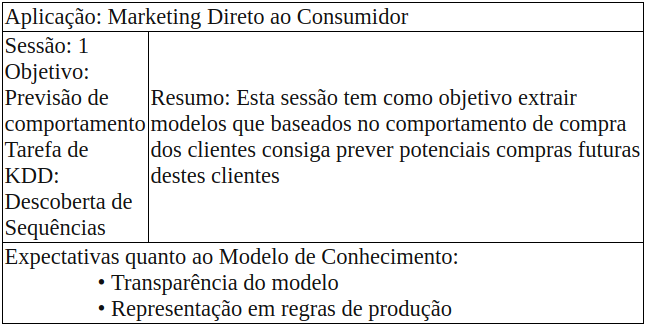
\includegraphics[scale=.4]{imagens/formulario-etapa-definicao-objetivo.png}
  \caption{Exemplo de preenchimento do formulário na etapa de Definição de Objetivos. Fonte: \cite{goldschmidt2015data}.}
  \label{fig:formulario-etapa-definicao-objetivo}
\end{figure}

\section{Planejamento de atividades}
\label{sec:planejamento-de-atividades}

Nesta etapa cada sessão de KDD identificada na sessão \ref{sec:definicao-dos-objetivos} deverá ser elaborado um planejamento de atividades que proporcione a execução do objetivo correspondente. Também será identificado, dentre o métodos disponíveis, aqueles que melhor implementam a tarefa da sessão de KDD. Este métodos são chamados de métodos candidatos.

Segundo \citet{goldschmidt2015data} a filtragem dos métodos requer conhecimento profundo de cada método e que a escolha do método depende da preferência pessoal do analista de KDD, porem ressalva que todos os métodos candidatos que não foram retirados da filtragem devem ser considerados. A filtragem dos métodos candidatos será feita junto aos orientadores e ao fim dessa filtragem será elaborado uma lista ordenada dos método que podem obter melhor resultado.

A partir da listagem dos métodos selecionados será apresentado alternativas de pré-processamento para cada método da lista. \citet{goldschmidt2015data} denomina essas alternativas de pré-processamento de planos de ação e que o analista deve planejar quais métodos de pré-processamento devem ser utilizados, incluindo a ordem de aplicação.

A figura \ref{fig:formulario-etapa-planejamento-atividades} é um exemplo retirado do livro que mostra como ficaria o formuláro após a etapa de planejamento de atividades.

\begin{figure}[htbp]
  \centering 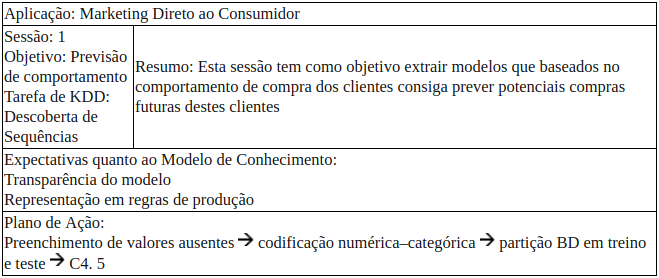
\includegraphics[scale=.4]{imagens/formulario-etapa-planejamento-atividades.png}
  \caption{Exemplo de preenchimento do formulário na etapa de Planejamento de Atividades. Fonte: \cite{goldschmidt2015data}.}
  \label{fig:formulario-etapa-planejamento-atividades}
\end{figure}

\section{Execução do Plano de Ação}
\label{sec:execucao-do-plano-de-acao}

Nesta etapa todos os planos de ação descritos na sessão \ref{sec:planejamento-de-atividades} serão experimentados e avaliados. \citet{goldschmidt2015data} recomenda que os planos sejam executados simultaneamente para ser feito uma análise conjunta dos resultados obtidos. Isso pode trazer uma visão global do processo e pode ser possível perceber detalhes que permitam reavaliar ou mudar a estratégia escolhida.

\citet{goldschmidt2015data} recomenda também que o plano de ação entende a execução ordenada dos métodos do plano e deve ser executada em ciclos. Ou seja, o plano deve ser executado total ou parcialmente a cada ciclo, procurando obter os melhores resultados.

\citet{goldschmidt2015data} destaca que um problema frequente em um processo de KDD é a escolha dos parâmetros de um algoritmo frente a uma nova situação. Este problema pode aumentar bastante o número de ciclos do processo. Por isso, nessa etapa serão registrados dos parâmetros adotados e os resultados obtidos a cada ciclo no formulário. A figura \ref{fig:formulario-etapa-execucao-dos-planos-de-acao} mostra um possível preenchimento do formulário.

\section{Avaliação de Resultados}
\label{sec:avaliacao-de-resultados}

Esta etapa deve ser realizada no final do processamento de cada método do plano. \citet{goldschmidt2015data} diz que é o momento de comparar as características do modelo de conhecimento gerado com as expectativas quanto ao modelo de conhecimento listadas na sessão \ref{sec:definicao-dos-objetivos}. Ele reforça que algumas medidas podem ser comparadas diretamente, já outras, são mais subjetivas. Uma pergunta que poderia se fazer nessa etapa é qual é a exclusividade e utilidade do conhecimento extraído? Por isso, esta etapa deverá ser homologada junto ao orientador deste trabalho. Nessa etapa também terá de ser feito um estudo sobre as medidas de interesse no processo de KDD.

\begin{figure}[htbp]
  \centering 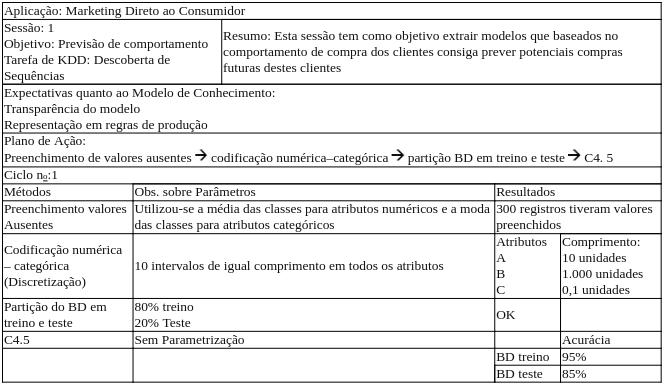
\includegraphics[scale=.4]{imagens/formulario-etapa-execucao-dos-planos-de-acao.png}
  \caption{Exemplo de preenchimento do formulário na etapa de Execução do plano de ação. Fonte: \cite{goldschmidt2015data}.}
  \label{fig:formulario-etapa-execucao-dos-planos-de-acao}
\end{figure}


% O processo de descoberta de conhecimento envolve várias fases e etapas. Para o desenvolvimento deste trabalho será utilizada a abordagem proposta por [Silva and Vieira 2002] e [Rezende et al. 2003] onde o processo pode ser separado em três fases: Preparação, Extração de Padrões e Pós-Processamento. Cada fase pode envolver uma ou mais etapas. No podem ser realizadas novamente após a análise dos padrões encontrados de forma a melhorá-los \cite{Pimentel2006}.

% Descoberta de conhecimento em base dados pode ser composto por várias etapas operacionais \cite{goldschmidt2015data}.
% Este trabalho será dividido em 3 grandes momentos: coleta dos dados, pré-processamento dos dados, criar e avaliar os modelos de predição.

% Na etapa de coleta será coletado todo o dado bruto referente aos alunos dos cursos de graduação da UFPEL. Esta etapa será feita de forma manual através de consultas a base de dados.
% Os sistemas de aplicações, conhecidos por OLTP (On-Line Transaction Processing), processam dados armazenados em Base de Dados relacionais usadas para armazenar, consultar e alterar informações do negócio. Normalmente, não é possível aplicar as técnicas de MD diretamente a estas bases, pois isso poderia resultar numa sobrecarga de consultas nas mesmas podendo literalmente “travar” um sistema, impossibilitando qualquer outro tipo de operação transacional. 
% Assim, é recomendável que os dados a serem utilizados na descoberta de conhecimento estejam separados da Base de Dados operacional. Nesses casos, utilização de DW é indicada, pois possibilita o armazenamento de grande quantidade de dados históricos de uma organização e viabiliza acessos otimizados aos dados previamente consolidados, reduzindo consideravelmente o tempo de realização do processo de MD \cite{Rezende2002}.

% Em seguida vem a etapa de pré-processamento onde será verificado a necessidade de fazer a limpeza e classificação dos dados para serem utilizados nos testes. Da mesma forma que a primeira esta etapa também sera feita de forma manual.

% De uma forma mais macro vem a terceira etapa onde será gerado um modelo de predição aplicando algoritmos de aprendizagem de máquina e posteriormente este modelo será avaliado a partir dos resultados.

% O processo de mineração de dados envolve várias fases e etapas. Este trabalho classifica o processo de KDD em três grandes fases, com base nas abordagens descritas em [Silva and Vieira 2002] e [Rezende et al. 2003]: Preparação, Extração de Padrões e Pós-Processamento. Cada fase pode envolver uma ou mais etapas conforme mostra a tabela 1. No entanto, o KDD é um processo iterativo e algumas etapas podem ser realizadas novamente após a análise dos padrões encontrados de forma a melhorá-los \cite{Pimentel2006}.



% Nesta seção, apresenta-se a metodologia proposta para o
% desenvolvimento da Dissertação. O proponente deve descrever as
% atividades necessárias para a conclusão dos objetivos propostos. 

\chapter{Cronograma}

Esta seção apresenta a relação de atividades que deverão ser realizadas e o seu  cronograma para finalização do mestrado em Março/2020. As atividades são as seguintes:

\begin{itemize}
\item Revisão Bibliográfica: trabalho já realizado e versou sobre descoberta de conhecimento ...;
\item Extração dos Dados: já em andamento consta da extração ...
\item ...
\item Escrita da  dissertação;
\item Escrita e submissão de artigo;
\item Entrega e defensa da dissertação.
\end{itemize}

Dessa forma, de acordo com a metodologia proposta, foram listadas as
seguintes atividades:
1. Estudar técnicas de otimização de memória para sistemas embarcados;
2. Seleção e/ou desenvolvimento de benchmarks para avaliação das arquiteturas;
3. Pesquisa e seleção de ferramentas para avaliação/simulação das arquiteturas
e dos modelos de memória (para caracterização de latência e consumo energético);
4. Avaliação dos benchmarks nas arquiteturas através das ferramentas
selecionadas;
6. Propor e avaliar técnicas específicas para a arquitetura de processadores
embarcados;


O cronograma é apresentado na Figura \ref{fig:cronograma} ao longo do tempo.
\begin{figure}[htbp]
  \centering 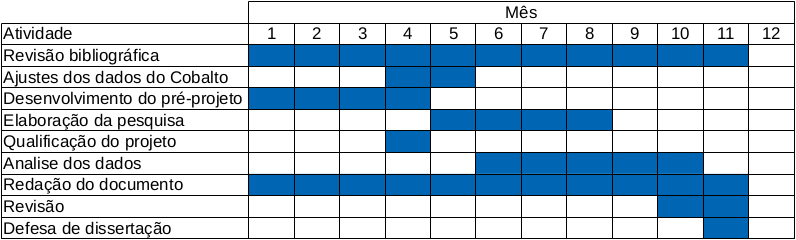
\includegraphics[scale=.4]{imagens/cronograma.png}
  \caption{Cronograma de atividades que serão realizadas.}
  \label{fig:cronograma}
\end{figure}

% Esta seção deve apresentar relação numerada de atividades (de estudo,
% modelagem, especificação, implementação ou validação) que deverão ser
% realizadas (incluindo atividades obrigatórias como seminário de
% andamento, entrega e apresentação da dissertação) e o cronograma
% destas atividades, distribuídas no prazo de 12
% meses.

\bibliography{bibliografia}
\bibliographystyle{abnt}

\chapter{Assinaturas}
\vspace{2cm}

\begin{center}
\rule{8cm}{.3mm}
\medskip

	Alexandre Gomes da Costa\\
	Proponente

\end{center}

\vspace{4cm}

\begin{center}
\rule{8cm}{.3mm}
\medskip

	Prof. Dr. Julio Carlos Balzano de Mattos\\
	Prof. Orientador

\end{center}
\end{document}
